\documentclass[12pt, a4paper]{article}
\linespread{1.54}
\pagestyle{myheadings}

\usepackage[T1]{fontenc}
\usepackage[utf8]{inputenc}
\usepackage{lmodern}
\usepackage{enumitem}
\usepackage{tabularx}
\usepackage[labelfont={footnotesize,bf} , textfont=footnotesize]{caption}
\captionsetup{labelformat=simple, labelsep=period}
\makeatother
\setlength{\intextsep}{10pt}
\setlength{\abovecaptionskip}{2pt}
\setlength{\belowcaptionskip}{-10pt}
\usepackage{cleveref}
\usepackage{graphicx}
\graphicspath{ {./} }
\usepackage[english]{babel}
\usepackage{csquotes}
\usepackage[export]{adjustbox}

\usepackage[notes, backend=biber]{biblatex-chicago}
\bibliography{PythonFinalReport.bib}
\usepackage{url}

\begin{document}
\title{Cox Proportional Hazard Models in Pystan:\\ \large{Repeating Karlen's Analysis}}
\author{Devin P. Brown}
\date{01 June 2020}
\maketitle
For my final project, I replicated Niklas Karlen's analysis in ``Turning off the Taps: The Termination of State Sponsorship.''\autocite{Karlen2019} First, I repeated his analysis in Python using a simple Cox Proportional Hazard Model. Then I coded the same model in Pystan. Finally, to improve his analysis, I added random effects for each supporting state to the simple pystan model. While my results in the first two replications broadly agree with Karlen's analysis, the addition of random effects significantly altered the results, causing the confidence intervals to sharply increase and switching the signs of three variables. This shows that random effects are the improper method to improve Karlen's analysis. In this report, I will detail my analysis, compare the results, and map out the future of this project. 

Karlen's article is a first attempt at quantitatively explaining when external states will terminate support for foreign rebel groups. He includes ten explanatory variables in his model. The first set of independent variables are simply the inverse of common explanations for support provision. These include (1) rivalry between the target and supporting state, (2) whether the target state is receiving support, (3) whether the sponsor state has kinship ties to the sponsored insurgent organization, (4) whether the supporting state is democratic, and (5) the end of the cold war. Perceiving that each of these variables are structural and relatively static, he then generates his five more potential short-term triggers for support termination: (6) leadership change in the supporting state, (7) an economic downturn in the sponsor state, (8) the outbreak of an armed conflict in the supporting state, (9) the threat of sanctions against the sponsor, and (10) actual sanctions against the supporter in response to its assistance to the insurgent group. He coded his dependent variable---support termination---based on when UCDP stopped coding external support. He includes other variables such as a lagged version of his government support indicator and another binary variable that tested the impact of previous terminations.

\begin{figure}[h]
	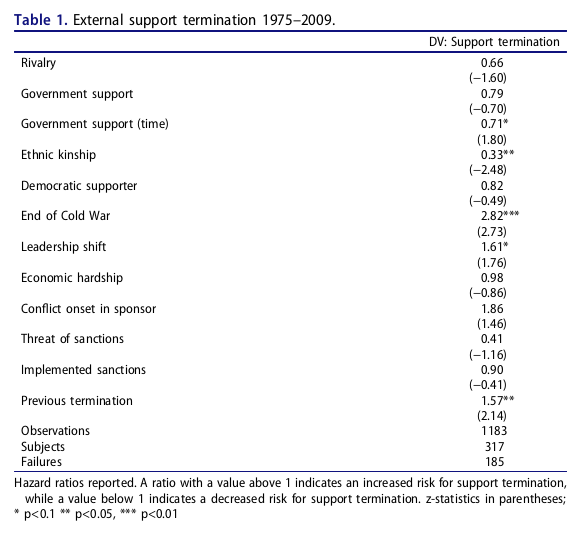
\includegraphics[width=0.9\textwidth]{KarlensResults}
	\centering
	\caption{Karlen's results reported as hazard ratios.} 
	\label{Karlen}
\end{figure}
		
Karlen then runs a Cox Proportional Hazard Regression including each of these variables with clustered standard errors on the sponsor. His central findings survived his robustness checks in which he used Weibull, Poisson, and logit distributions. His results can be seen in \Cref{Karlen}. He finds strong negative support for kinship and positive support for the end of the Cold War, that is ethnic kinship discourages support termination while the end of the Cold War encourages termination. Regarding triggers, none of his findings were robust to different specifications. In general, testing all variables in one model is bad practice, especially considering that some of his variables are not mutually independent. This clouds his ability to clearly distinguish the effect of each variable. 

\begin{figure}[h] 
	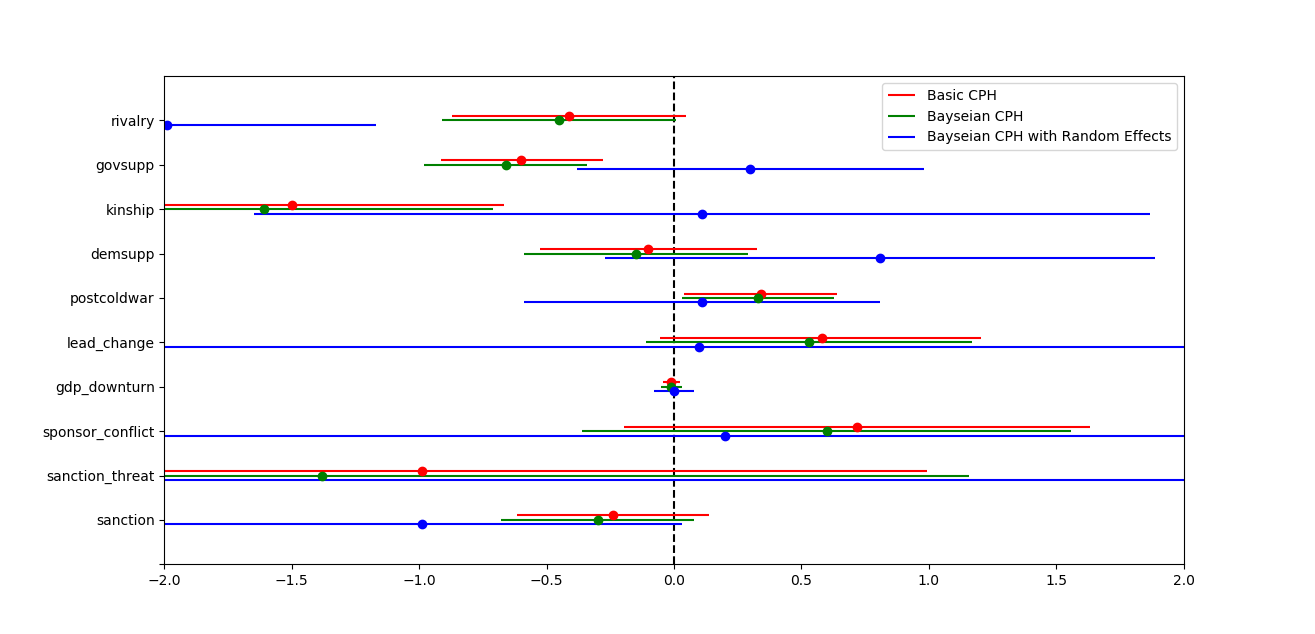
\includegraphics[width=1.3\textwidth, center]{CI_Chart}
	\centering
	\caption{Replication Results as coefficients.}
	\label{Me}
\end{figure}

The author was kind enough to send me his dataset, enabling me to replicate his analysis. First, I used a simple Cox Proportional Hazard model. I then coded the same model in Pystan. Neither of these replications included any extra specifications or standard error clustering.  The results from these two are nearly identical to Karlen's analysis. Each of my variables maintained the same sign and achieved similar levels of significance. However, both of my models found stronger correlations with government support as can be seen in \Cref{Me}. I then added random effects to the Pystan model since the use of clustered standard errors has been proven to harm analyses.\autocite{King2015} I placed very strict priors on the distribution of the average and variance of both censored and uncensored data groups because early trials returned astronomical standard errors. Pystan itself warned that the model was misspecified. Despite these stricter priors, the inclusion of random effects consumed most of the model's variation, clearly illustrating that random effects is an improper method to improve this analysis. The final model still included extremely broad standard errors and returned very uninformative results. In fact, only rivalry seems to correlate strongly with support continuation. Otherwise, compared to Karlen's study, kinship, government support, and democracies changed sign yet failed to disprove the null hypothesis. 

In the future, I will continue this analysis to better pinpoint reasons why states terminate support to insurgent groups. First, I will use San-Akca's dataset, NAGS,\autocite{SanAkca2016} since it includes a coded measure for support termination which only includes acts of overt suspension of assistance. Second, I will use Karlen's structural variables to calculate the baseline hazard, better pinpointing the effect of his triggers. Finally, I will draw from Popovic's 2017 article and test the effect of defection on support termination.\autocite{Popovic2017} This is a better researched and more theoretically grounded potential trigger for the dependent variable of interest. Ultimately, I intend to submit this new test for publication and contribute to this nascent research agenda.

\newpage
\printbibliography
\end{document}